\chapter{\IfLanguageName{dutch}{Stand van zaken}{State of the art}}
\label{ch:stand-van-zaken}

% Tip: Begin elk hoofdstuk met een paragraaf inleiding die beschrijft hoe
% dit hoofdstuk past binnen het geheel van de bachelorproef. Geef in het
% bijzonder aan wat de link is met het vorige en volgende hoofdstuk.

% Pas na deze inleidende paragraaf komt de eerste sectiehoofding.


\color{blue}
Dit hoofdstuk bevat je literatuurstudie. De inhoud gaat verder op de inleiding, maar zal het onderwerp van de bachelorproef *diepgaand* uitspitten. De bedoeling is dat de lezer na lezing van dit hoofdstuk helemaal op de hoogte is van de huidige stand van zaken (state-of-the-art) in het onderzoeksdomein. Iemand die niet vertrouwd is met het onderwerp, weet nu voldoende om de rest van het verhaal te kunnen volgen, zonder dat die er nog andere informatie moet over opzoeken \autocite{Pollefliet2011}.

Je verwijst bij elke bewering die je doet, vakterm die je introduceert, enz. naar je bronnen. In \LaTeX{} kan dat met het commando \texttt{$\backslash${textcite\{\}}} of \texttt{$\backslash${autocite\{\}}}. Als argument van het commando geef je de ``sleutel'' van een ``record'' in een bibliografische databank in het Bib\LaTeX{}-formaat (een tekstbestand). Als je expliciet naar de auteur verwijst in de zin, gebruik je \texttt{$\backslash${}textcite\{\}}.
Soms wil je de auteur niet expliciet vernoemen, dan gebruik je \texttt{$\backslash${}autocite\{\}}. In de volgende paragraaf een voorbeeld van elk.

\textcite{Knuth1998} schreef een van de standaardwerken over sorteer- en zoekalgoritmen. Experten zijn het erover eens dat cloud computing een interessante opportuniteit vormen, zowel voor gebruikers als voor dienstverleners op vlak van informatietechnologie~\autocite{Creeger2009}.

\color{black}

\section{Verkennend onderzoek}
\label{sec:verkennend-onderzoek}
``Kan \textit{elderspeak} gedetecteerd worden door Artificiële Intelligentie en kan dit toegepast worden in de praktijk?'', is de centrale onderzoeksvraag, maar daarvoor moeten we twee begrippen goed uitleggen en begrijpen om te kunnen staven of dit wel degelijk mogelijk is.
Er zal dus eerst beschreven worden wat \textit{elderspeak} precies is. Waarom vinden ouderen dat niet leuk? Wat zijn de eigenschappen en hoe kan je het voorkomen?
Daarnaast moeten we ook begrijpen wat Artificiële Intelligentie is. De reden hiervoor is dat er verstaan moet worden wat dat is, welke types er zijn en hoe dit gebruikt werd het eindresultaat.

\section{Elderspeak}

\subsection{Wat is \textit{Elderspeak}?}

Het begrip \textit{elderspeak}, ook \textit{secondary babytalk} genoemd, kent verschillende definities. \textcite{Kemper_1998} omschrijft het begrip als volgt:
"Elderspeak is a simplified speech register with exaggerated pitch and intonation, simplified grammar, limited vocabulary and slow rate of delivery.”

Daarnaast beschrijft \textcite{Williams2011} het begrip als het volgende:
“Elderspeak is a common intergenerational speech style used by younger persons in communication with older adults in a variety of community and health care settings. Based on negative stereotypes of older adults as less competent communicators, younger speakers (in this case nursing home staff) modify their communication with nursing home residents by simplifying the vocabulary and grammar and by adding clarifications such as repetitions and altered prosody.”

\subsection{Wat zijn de kenmerken?}
Deze kenmerken komen overeen met een communicatiestijl die men hanteert wanneer men tegen (afhankelijke) kinderen praat. Vandaar dat \textit{elderspeak} ook wel als \textit{secondary baby} talk wordt benoemd.

\begin{itemize}
    \item Langzaam spreken
    \item Verhoogde toonhoogte
    \item Verhoogd stemvolume
    \item Overdreven intonatie
    \item Vereenvoudigd woordgebruik, gebruik van verkleinwoorden en/of ongepaste bijnamen of troetelnamen
    \item Verminderde grammaticale complexiteit (bv. voornamelijk enkelvoudige zinnen)
    \item Gebruik van collectieve voornaamwoorden (bijvoorbeeld “we” in plaats van “jij”)
    \item Veelvuldig gebruik van (bevestigende) tussenwerpsels (zoals “hé” of voilà”)
    \item Gewijzigd non-verbaal gedrag (bv. langdurig oogcontact, extra gebaren, te dichtbij komen)
    \item Veelvuldige verduidelijking en herhaling
\end{itemize}

Tenslotte is het belangrijk om te weten dat bij elderspeak de inhoud van de boodschap, die de zorgverlener wil overbrengen, niet wijzigt. Wel verandert de wijze waarop de boodschap wordt overgebracht door het gebruik van een infantiliserende communicatiestijl, aldus \textcite{Campens21}.

\subsection{Wat zijn de tips om \textit{elderspeak} te voorkomen?}

De onderstaande tips zijn enkele van de tips die \textcite{Wick2007} meegeven ter ``bestrijding'' van \textit{elderspeak}:

\begin{itemize}
    \item Spreek personen aan met de naam waarmee ze willen aangesproken worden. Gebruik geen collectieve voornaamwoorden als die niet van toepassing zijn.
    \item Als een persoon een zorgverlener toelaat om hem of haar met zijn voornaam aan te spreken, ga er dan niet van uit dat deze “toestemming” voor alle zorgverleners geldt. De mate van intimiteit varieert, waardoor elke zorgverlener moet nagaan hoe hij of zij zijn gesprekspartner mag aanspreken.
    \item Vermijd het gebruik van troetelnamen en overmatige intieme liefkozingen, tenzij de gesprekspartner uitdrukkelijk aangeeft dat hij of zij zo wil aangesproken worden.
    \item Wees je bewust van je non-verbaal gedrag.
    \item Verhoog je stemvolume (in beperkte mate) enkel en alleen wanneer de gesprekspartner hardhorig is. Verhoging van je stemvolume betekent geen verhoging van je stemhoogte. Wees je ervan bewust dat niet elke oudere gesprekspartner hardhorig is.
    \item Herhaling en verminderde grammaticale complexiteit hebben een plaats als de gesprekspartner je niet begrepen heeft.
    \item Vermijd korte zinnen en langzaam en met overdreven intonatie uitgesproken zinnen.
    \item Vermijd het gebruik van verkleinwoorden, aangezien die het gevoel van afhankelijkheid kunnen versterken en denigrerend kunnen geïnterpreteerd worden.
    \item Vermijd overdreven directieve boodschappen en bied keuzevrijheid.
    \item Hanteer een beleefd taalgebruik en beleefde omgangsvormen (bv. op de kamerdeur kloppen alvorens de kamer binnen te gaan).
\end{itemize}

\section{Artificiële Intelligentie}
\subsection{Wat is AI?}
Er zijn bijzonder veel beschrijvingen rond wat AI is, maar alleen uit verschillende bronnen kan je een accuraat beeld krijgen van wat AI is.

Volgens \textcite{Oracle2014} heeft AI (kunstmatige intelligentie) betrekking op systemen of machines die onze eigen intelligentie nabootsen om taken uit te voeren en die zichzelf tijdens dat proces kunnen verbeteren op basis van de vergaarde informatie.

Het \textcite{EuropeesParlement2020} geeft de volgende definitie van artificiële intelligentie (of kunstmatige intelligentie): ``AI is de mogelijkheid van een machine om mensachtige vaardigheden te vertonen - zoals redeneren, leren, plannen en creativiteit.
AI maakt het voor technische systemen mogelijk om hun omgeving waar te nemen, om te gaan met deze waarnemingen en problemen op te lossen om een specifiek doel te bereiken. De computer ontvangt data - reeds voorbereid en verzameld via eigen sensoren, zoals een camera - verwerkt deze en reageert erop.
AI-systemen zijn in staat om hun gedrag in zekere mate aan te passen, door het effect van vorige acties te analyseren en autonoom te werken.''

Samengevat is AI een technisch systeem om onze eigen intelligentie na te bootsen op basis van vergaarde informatie en waarbij het systeem acties aanpast op die data.

\subsection{Welke vormen zijn van AI?}
Artificiële Intelligentie is een verzamelnaam voor 2 soorten. Zo heb je enerzijds \textit{machine learning} en anderzijds \textit{deep learning} \autocite{Kavlakoglu2020}.
Dit kan mooi geïllustreerd worden a.d.h.v. figuur \ref{fig:soorten_ai_diagram}. Daarop kan er afgeleid worden dat Artificiële Intelligentie een verzamelnaam is. Specifieker heb je dan \textit{machine learning} en daaronder heb je nog \textit{deep learning}.

\begin{figure}
    \centering
    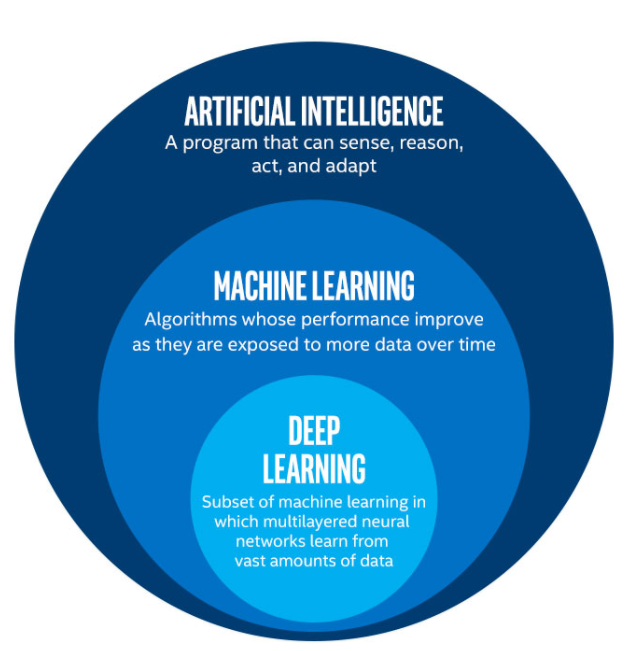
\includegraphics[width=0.5\textwidth]{./img/ai_fields.png}
    \caption{\label{fig:soorten_ai_diagram} Soorten AI in diagram \autocite{Bansal2019}}
\end{figure}

\subsection{\textit{Machine learning}}
\textit{Machine learning} of machinaal leren is het deelgebied van kunstmatige intelligentie dat computers het vermogen geeft te leren zonder expliciet geprogrammeerd te zijn, aldus \textcite{Lievens2021}. Machinaal leren heeft drie types namelijk \textit{supervised learning} of gesuperviseerd leren, \textit{unsupervised learning} of leren zonder toezicht en als laatste type is er \textit{reinforcement learning} of leren door bekrachtiging.

\subsubsection{Supervised learning}
Een defenitie gegeven door \textcite{Lievens2021} over \textit{supervised learning} gaat als volgt: ``De taak van \textit{supervised learning} is een hypothese op te bouwen op basis van een reeks gelabelde trainingsgegevens. Deze hypothese kan dan worden gebruikt om het label voor een (nieuwe) input te voorspellen. Wanneer het label een reëel getal is, spreekt men van een regressieprobleem; wanneer het label beperkt is tot één van een (beperkt) aantal vooraf gedefinieerde klassen, wordt het probleem een classificatieprobleem genoemd.''

Een voorbeeld van het regressieprobleem is het voorspellen van huisprijzen. De input van het model is dan een reeks vectoren die de eigenschappen van het huis voorstellen zoals aantal slaapkamers, oppervlakte, bouwjaar etc.
Voorbeelden van het classificatieprobleem zijn spam detectie of nummerherkenning. Bij spam dectactie heb je twee vooraf gedefinieerde klassen: spam en geen spam. Bij het herkennen van nummers heb je 10 klassen: 0 t.e.m. 10.

\subsubsection{Unsupervised learning}
\textcite{Lievens2021} omschrijft \textit{unsupervised learning} als de taak van een algoritme voor leren zonder toezicht is het ontdekken van structuur te ontdekken in een ongelabelde gegevensreeks. De meest prominente taak bij \texit{unsupervised learning} is clustering, d.w.z. de ontdekking van coherente
groepen. Andere mogelijke taken zijn anomalie detectie en hoofdcomponentenanalyse (PCA).

Een voorbeelden van clustering is markt segmentatie waarbij klanten worden opgedeeld in verschillende segmenten zoals trouwe klant, mogelijke vertrekkende klant, niet tevreden klant etc.
Je hebt algoritmen die fraude opsporen op een website die dus vreemd gedrag gaan detecteren. Dit is dan een voorbeeld van anomalie detectie.
Bij PCA worden de data gereduceerd zodat de minder relevante data afneemt in de dataset.


\subsubsection{Reinforcement learning}
\textcite{Lievens2021} beschrijft leren door bekrachtiging door een techniek dat niet echt een dataset gebruikt, maar dat het eerder een identiteit is die leeft in een (on)bekende wereld die beloningssignalen krijgt. De opdracht is dan om uit te zoeken wat de regels zijn die leiden tot een grote beloning.

Het bekendste voorbeeld van \textit{reinforcement learning} is zelfrijdende wagens waarbij het model alles zelf moet aanleren zoals het remmen en gas geven in welke hoeveelheid en hoe er gestuurd moet worden.

\subsection{Deep Learning}

``Een artificieel neuraal netwerk bestaat uit een groot aantal eenvoudige rekende eenheden, units of neuronen die de volgende eigenschap heeft: Als de (gewogen) input van een neuron groot is, zal het "vuren" en dit neuron zal een grote waarde op zijn axon zetten. Bovendien zijn deze eenheden verbonden door middel van gerichte links waarbij een reëel getal de sterkte van elke verbinding aangeeft.'', aldus \texcite{Lievens2021} in zijn cursus \textit{Distributed Databases}.

De systematische voorstelling van een neuron is te vinden in figuur \ref{fig:neuron}.
Een volledig neuraal netwerk kan er uit zien zoals in figuur \ref{fig:layers}

\begin{figure}
    \centering
    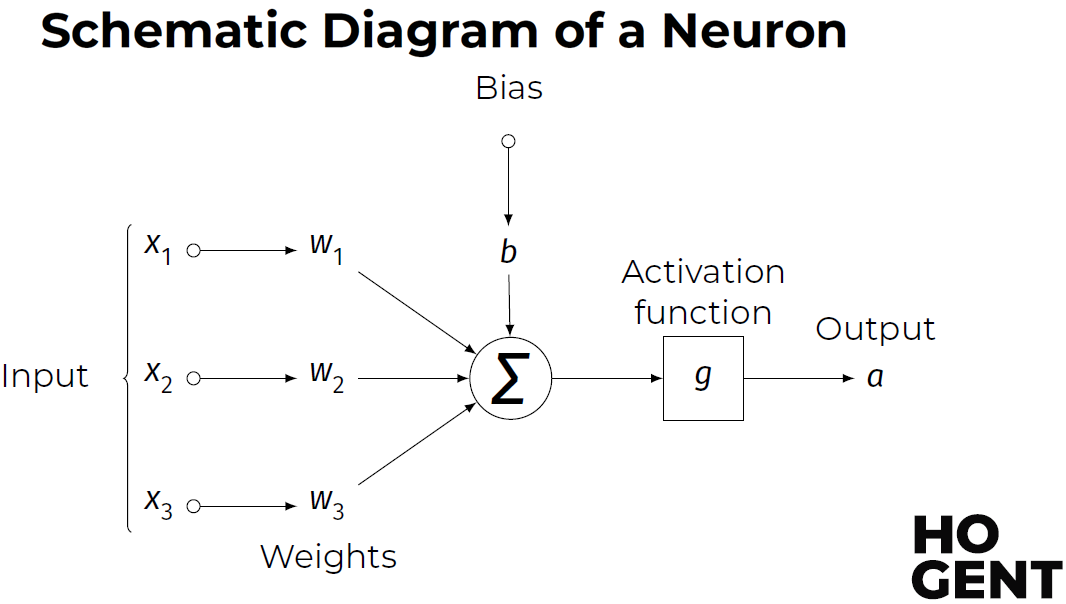
\includegraphics[width=1\textwidth]{./img/neuron.png}
    \caption{\label{fig:neuron} Systematische voorstelling van een Neuron \autocite{Lievens2021}}
\end{figure}

\begin{figure}
    \centering
    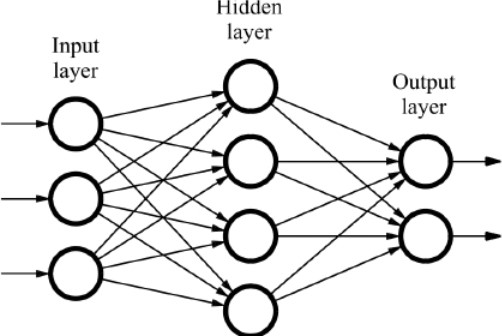
\includegraphics[width=1\textwidth]{./img/layers.jpg}
    \caption{\label{fig:layers} Layers van een artificieel neuraal netwerk \autocite{Lievens2021}}
\end{figure}

\subsection{AI in het dagelijkse leven}
Om een klein overzicht te maken wat AI allemaal inhoudt, zijn er andere voorbeelden geïllustreerd van kunstmatige intelligentie in figuur \ref{fig:ai_dagelijkse_leven}.
\begin{figure}
    \centering
    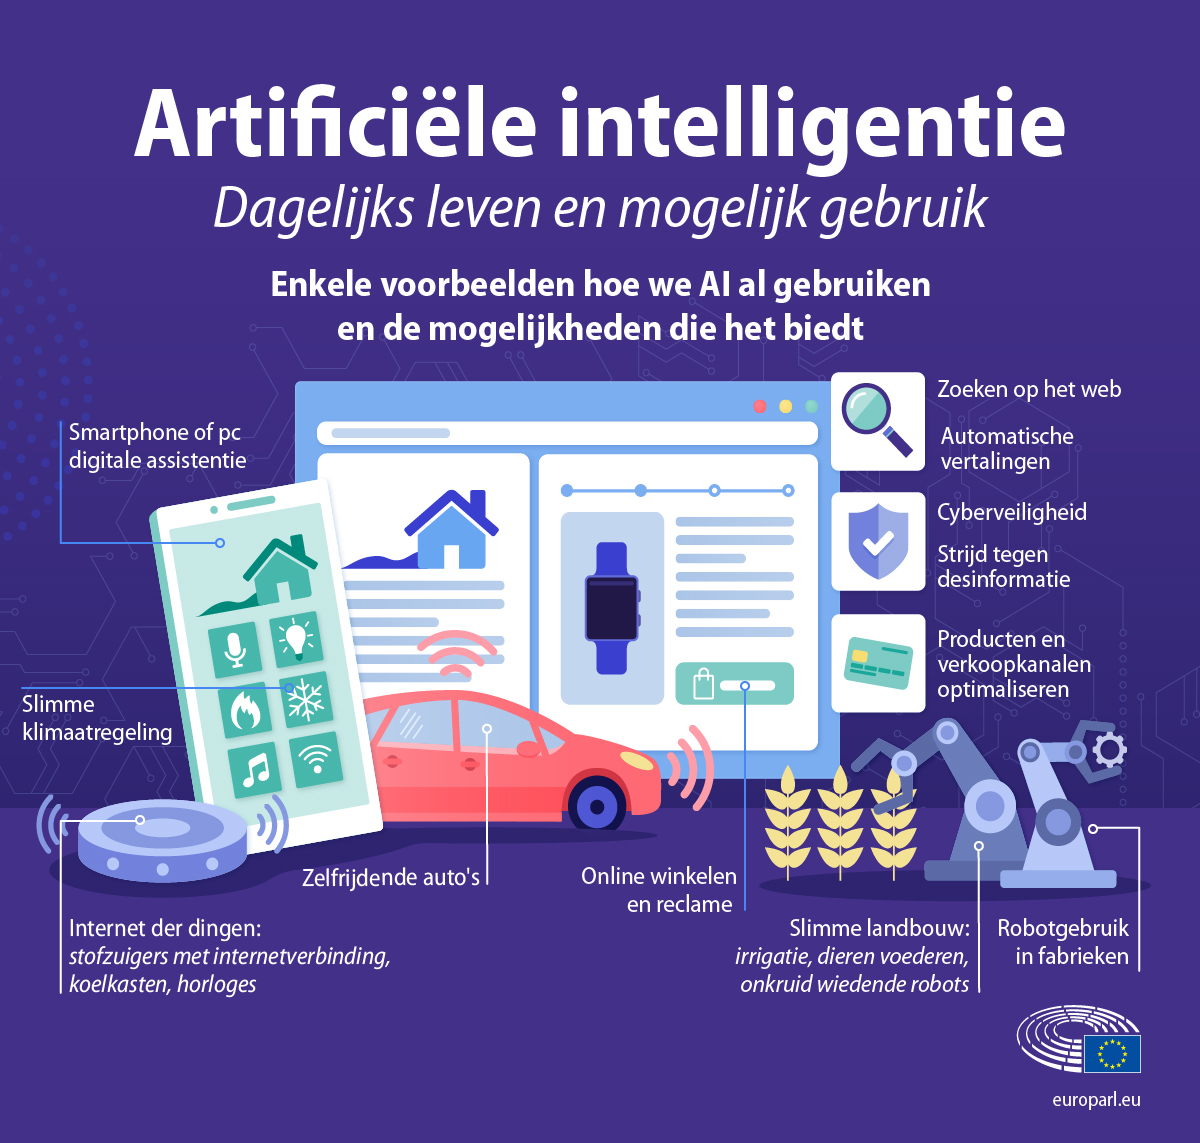
\includegraphics[width=0.5\textwidth]{./img/ai_voorbeelden.jpg}
    \caption{\label{fig:ai_dagelijkse_leven} AI in het dagelijkse leven. \autocite{EuropeesParlement2020}}
\end{figure}

\section{AI technieken die gebruikt worden om elderspeak te detecteren}
\subsection{Google Text-to-Speech}